\documentclass[a4paper,graphics,11pt,notitlepage]{scrartcl}

\usepackage{graphicx,curves,epsf,float,rotating}
\usepackage{epsf,epsfig,eepic}
\usepackage{latexsym,amsmath,amssymb}
\usepackage[utf8]{inputenc}
\usepackage{theorerms}
\usepackage{dcolumn}
\usepackage{tikz}
\usepackage{pgfplots}
\usepackage{enumerate}
\usepackage{enumitem}
\usepackage{footnote}
%\usepackage{biblatex}
\usepackage{fancyhdr}
\usepackage[english]{babel}
\usepackage{listings}
\lstset{
  basicstyle=\ttfamily,
  columns=fullflexible,
  frame=single,
  breaklines=true,
  postbreak=\mbox{\textcolor{red}{$\hookrightarrow$}\space},
}

\usepackage[
colorlinks=false,
bookmarksnumbered = true,
linkbordercolor= white,
citebordercolor= white,
urlbordercolor= white]{hyperref}



%\textwidth 15cm
%\textheight 23cm
%\oddsidemargin 1cm
%\evensidemargin 0cm
%\parindent 0mm

\title{Solutions to Sheet 5}
\author{Friedrich May, 355487; Markus Moll, 406263; Mariem Mounir, 415862\\Group 57}

\begin{document}
  \vspace{-5ex}
  \maketitle
  \section*{Exercise 1}
To calculate the class for every point we first need to find the $k$ closest points (depending on the norm).
To archive this, a script like the following can be used:
\lstinputlisting[language=matlab]{knn.m}
Using the results the following table can be created. Note that the ties can be arbirarily chosen.


  \centering \begin{tabular}{l|c|c|c|c}
    Norm&\multicolumn{2}{c}{Euclidian}&\multicolumn{2}{c}{Manhattan}\\\hline
    k&2&3&2&3\\\hline
    4,3,3&1&1&1&1\\
    4,-1,1&1(tie)&-1&1(tie)&1\\
    -2,4,5&-1&-1&1(tie)&1\\
    -2,-6,1&1(tie)&1&1(tie)&1\\
    6,0,2&1(tie)&1&-1&-1
  \end{tabular}

\flushleft
  \section*{Exercise2}
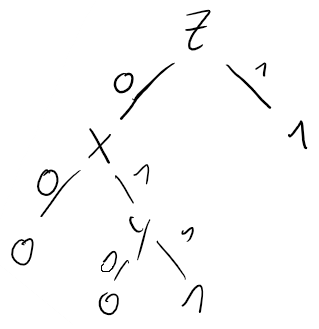
\includegraphics[scale=0.5]{E2Tree.png}

The first split is done using $z$, because this is the only variable for wich the result stays the same for a value of the variable.
The other two splits could be swapped because the influence on the result is the same for both variables.
  %
\section*{Exercise 3}

\subsection*{a)}  % This is meant to be a section heading

We have \[S=((x_{1},y_{1}), ..., (x_{k},y_{k}))\]  with \[x_{i}\in \left \{ -1, 1 \right \}^{n} , y_{i}\in \left \{ -1, 1 \right \} \forall i\in [k]\]

Let p be the number of updates needed for the Perceptron Algorithm. 

So we have (1) : \[\left \langle w_{p},x_{i}y_{i} \right \rangle\geq 0 \  \forall i\in [k]\] 

And we have also : \[w_{p}-w_{p-1}=x_{p-1}y_{p-1}\]
So : 
\[\left \langle w_{p}-w_{p-1},x_{p-1}y_{p-1} \right \rangle=\left \langle x_{p-1}y_{p-1}, x_{p-1}y_{p-1}\right\rangle\]
\[\left \langle w_{p}-w_{p-1},x_{p-1}y_{p-1} \right \rangle=n\]
\[\left \langle w_{p},x_{p-1}y_{p-1} \right \rangle - \left \langle w_{p-1},x_{p-1}y_{p-1} \right \rangle=n\]
Using (1) we have :\[\left \langle w_{p-1},x_{p-1}y_{p-1} \right \rangle + n \geq 0 \]
\[\left \| w_{p-1} \right \| \left \| x_{p-1}y_{p-1} \right \| + n \geq \left \langle w_{p-1},x_{p-1}y_{p-1} \right \rangle + n \geq 0\]

And we saw in the lecture that for each $i\leq p-1$ :

\[\left \| w_{i} \right \| \leq \sqrt{i}\]
 Thus :
 \[n+ n^{2}(p-1) \geq n+ n^{2}\sqrt{p-1}\geq 0\]
Finally:
\[1-\frac{1}{n}\leq p\]

 

\subsection*{b)}
We have that the function: \[maj(x_{i})=\begin{cases} 1 & \text{ if } \sum_{j=1 }^{n}x_{ij}> 0 \\ -1 & \text{ else } \end{cases}\]

If we have $\sum_{j=1 }^{n}x_{ij}> 0$, we need to find $w$ such as  \[\left \langle w,x_{i} \right \rangle\geq 0 \  \forall i\]
\[\left \langle w,x_{i} \right \rangle =\sum_{j=1}^{n}w_{j}x_{ij}\]
for w=(1,..,1) we have \[\left \langle w,x_{i} \right \rangle =\sum_{j=1 }^{n}x_{ij}> 0\]

We need to normalize this w, so finally our normalized vector w is :\[w=(\frac{1}{n},...,\frac{1}{n})\]

To find an upper bound on the number of updates of w the Perceptron Algorithm performs for any training set for the function maj, we need to find the margin: \[min_{(x,y)\in S}\left | \left \langle w,x \right \rangle \right |\]
And S is a normalised set
 We have for each p: 
 \[\left | \left \langle w,x_{p} \right \rangle \right |=\left | \sum_{j=1}^{n} \frac{x_{pj}}{n^{2}} \right |\]
 And because n is an odd number so will must have :
 \[\frac{1}{n^{2}}\leq \left | \sum_{j=1}^{n^{2}} \frac{x_{pj}}{n^{2}} \right |\]

So we found a lower bound, we just need to find a vector that  verify  it, and a vector that have the majority positive or negative by 1 elements verify it.

So the margin is: \[\gamma =\frac{1}{n^{2}}\]
Thus ( using theorem 1.10) we find that the upper bound is : 
\[n^{4} =\frac{1}{\gamma^{2}}\]
 
\subsection*{ c)}
 Yes, we will still find a linear separator that realizes maj. Because the Perceptron Algorithm has no restriction on the set. 
  

  \section*{Exercise 4}
\subsection*{a)}
Compute $S$: 
\[\left(\begin{matrix}
0&1&1&0&0&0&0&0&0\\1&0&1&1&0&0&0&0&0\\1&1&0&0&0&0&1&0&0\\
0&1&0&1&0&1&0&0&0\\0&0&0&1&0&1&0&0&0\\
0&0&0&1&1&0&0&1&0\\0&0&1&0&0&0&0&1&1\\0&0&0&0&0&1&1&0&1\\
0&0&0&0&0&0&1&1&0
\end{matrix}\right)\]
$L=D-S$
\[D=\left(\begin{matrix}
2&0&&&\cdots&&&&0\\
0&3&0\\&0&2&0\\&&0&3&0\\\vdots&&&0&2&0&&&\vdots\\&&&&0&3&0\\&&&&&0&3&0\\&&&&&&0&3&0\\0&&&&\cdots&&&0&2
\end{matrix}\right)\]
\[L=\left(\begin{matrix}
2&-1&-1&0&0&0&0&0&0\\-1&3&-1&-1&0&0&0&0&0\\-1&-1&2&0&0&0&-1&0&0\\
0&-1&0&2&0&-1&0&0&0\\0&0&0&-1&2&-1&0&0&0\\
0&0&0&-1&-1&3&0&-1&0\\0&0&-1&0&0&0&3&-1&-1\\0&0&0&0&0&-1&-1&3&-1\\
0&0&0&0&0&0&-1&-1&2
\end{matrix}\right)\]

\subsection*{b)}
The calculation of the eigenvalues of $L$ yielded the eigenvalues 0,0.6972,0.6972,3,3,3,4.3028,4.3028,5.
The three smallest eigenvalues therefore are $\lambda_1=0,\lambda_2=0.6972 \text{and} \lambda_3=0.6972$.
The corresponding eigenvectors are \\$e_1 = (-1/3\;-1/3\;-1/3\;-1/3\;-1/3\;-1/3\;-1/3\;-1/3\;-1/3)^T$, $e_2=(-0.2331\:-0.2605\:-0.0432\:-0.3234\:-0.3507\:-0.1335\:0.3940\:0.3666\:0.5838)^T$, $e_3 = (0.5396\:0.3046\:0.3984\:-0.2367\:-0.4717\:-0.3778\:0.0733\:-0.1617\:-0.0679)^T$
\subsection*{c)}
From the eigenvectors the matrix $U$ can be derived\[U=\left(\begin{matrix}
-0.3333&  -0.2331&0.5396\\
-0.3333&	-0.2605&	0.3046\\
-0.3333&	-0.0432&	0.3984\\
-0.3333&	-0.3234&	-0.2367\\
-0.3333&	-0.3507&	-0.4717\\
-0.3333&	-0.1335&	-0.3778\\
-0.3333&	0.3940&	0.0733\\
-0.3333&	0.3666&	-0.1617\\
-0.3333&	0.5838&	-0.0679\\
\end{matrix}\right)\]

Splitting the rows of $U$ using k-Means clustering yields the clusters\\ $\lbrace U_1,U_2,u_3\rbrace,\lbrace U_4,U_5,U_6\rbrace,\lbrace U_7,U_8,U_9\rbrace$.
  \section*{Exercise 5}
\subsection*{a)}

if $A = BB^T$:
observe that $A$ i s symmetric.
 \[x^TAx = x^TBB^Tx = (B^Tx)^TB^Tx = ||B^Tx|| \ge 0\]
 so $A$ is psd.
 
 
if $A$ is psd:
THere is an orthogonal matrix $U$ such taht $A=UDU^T$ with $D=\text{diag}(\lambda_1,\cdots,\lambda_n)$.
We can write $D=R\times R$ with $R=\text{diag}(\sqrt{\lambda_1},\cdots,\sqrt{\lambda_n})$.
So \[A=UR\times RU^T = UR(UR)^T\].
So there is a $B = UR$ such that $A = BB^T$.

\subsection*{b)}
Let $A = \left(\begin{matrix}
1&2\\2&1
\end{matrix}\right)$.
$A$ is not psd because $\left(\begin{matrix}
-1 & 1
\end{matrix}\right)A\left(\begin{matrix}
-1 & 1
\end{matrix}\right)^T = -2 < 0$.

  \section*{Exercise 6}


With $\alpha=\frac{1}{2}$, the event sequence 121234 and \[L=
\begin{pmatrix}
1 & 1 & 0 & 0\\ 
0 & 1 & 1 & 1\\ 
1 & 0 & 1 & \frac{1}{2}
\end{pmatrix}
\]


\subsection*{a)} Using the MWU algorithm, we find :


\begin{itemize}
    \item $\omega^{(1)} = (1,1,1)$
    \item $\omega^{(2)} = (\frac{1}{2},1,\frac{1}{2})$
    \item $\omega^{(3)} = (\frac{1}{4},\frac{1}{2},\frac{1}{2})$
    \item $\omega^{(4)} = (\frac{1}{8},\frac{1}{2},\frac{1}{4})$
    \item $\omega^{(5)} = (\frac{1}{16},\frac{1}{4},\frac{1}{4})$
    \item $\omega^{(6)} = (\frac{1}{16},\frac{1}{8},\frac{1}{8})$
    \item And finally : $\omega^{(7)} = (\frac{1}{16},\frac{1}{16},0.09)$
\end{itemize}

\subsection*{b)} Using the definition of the probability distribution, we find : 

\begin{itemize}
    \item The probability to follow the advice of expert 1 in round 6 is 0.2
    \item The probability to follow the advice of expert 2 in round 6 is 0.4
    \item The probability to follow the advice of expert 3 in round 6 is 0.4
\end{itemize}

So : $p^{(6)}=(0.2,0.4,0.4)$

\subsection*{c)}
Even if we change the order the result of $\omega^{(7)}$ will stay the same, because it does not depend on the order :
\[\omega_{i}^{(t+1)}=(1-\alpha )^{\sum_{s=1}^{t}L_{ij(s)}}\omega _{i}^{(1)}\]

\end{document}